\documentclass{entcs} 
\usepackage{CSC8498macro}
\usepackage{graphicx}
\graphicspath{{./Images/}}

%% This document describes the formatting instructions for the CSC8498 final report.

\makeatletter

\def\lastname{Boulderstone}
\begin{document}

\begin{frontmatter}
\title{Rollback Netcode, Implmentation and Adoption}
\author{Edward Boulderstone}
  \address{School of Computing Science, Newcastle University, UK} 
\thanks[nigellemail]{Email:
    \href{mailto:E.Boulderstone@ncl..ac.uk} {\texttt{\normalshape
        E.Boulderstone@ncl..ac.uk}}}

			
				
\begin{abstract} 
Rollback netcode is a peer to peer networking soultion. It had potential to improve online experiences by minimizing the effects of latency over traditional delay based . However the implementation of rollback netcode in the fighting game industry has been slow and difficult. This project aims to understand  understand how the industry has had difficulty implementing rollback, and find any optimizations that can be made to existing public rollback netcode understanding.
\end{abstract}

\begin{keyword}
rollback, netcode, peer to peer, fighting games, networking, industry.
\end{keyword}
\end{frontmatter}

\section{Introduction}\label{sec: introduction}
The goal of networking in video games is to allow people from all over the world to play with each other. However fans of fighting games have historically (Before the pandemic) gone out of their way to organise local tournaments with most major tournaments before the pandemic taking place off-line\cite{FGCMajors}. This trend started because of the when fighting games were played in arcades in the mid 1990's,\cite{FirstUSTournament} and continued until the start of the pandemic, in part because fighting games rely on consistent timing and a low latency environment \cite{DelayVsRollback}, \cite{BadNetcode}. The existing networking solutions at the time simply did not provide this environment for competitive play\cite{FGCAsEsport}. However the spread of the corona virus in the mid 2020's fighting games found themselves having to fall back onto these "lower quality" online platforms. Games which did not have well optimized netcode found themselves on the back foot, with reduced attention \cite{SmashTournamentsInThePandemic}, and games with well written netcode found their success  \cite{GuiltyGearStriveInThePandemic}.

\subsection{Delay Based Netcode}
The first solution to online play for fighting games was a peer to peer system known as delay based netcode. Peer to peer netcode is important for fighting games because of the aforementioned need for low latency. Because most fighting games are between two players \cite{FightingGameDefine}, introducing a server will increase the ping between the two players, as the information has to travel to a seperate location, before being sent to the opposing player. Delay based netcode works by keeping two players games identical, by waiting for the remote player's input, before running the game update

\subsection{Rollback Netcode}
Rollback netcode was developed in 2006 as a solution to the problems with delay based netcode. \cite{RollbackDevelopment}. It works on top of existing delay based netcode by adding rollback frames, predicting the remote users inputs. When the remote user's input arrives if it matches with the predicted input, nothing happens, however if there's a discrepancy the game will "rollback", to the point of the discrepancy and re-simulate the game state back to the real time frame as shown in figure \ref{fig:RollbackNetcodeRepresentation}.

\begin{figure}[h]
\centering
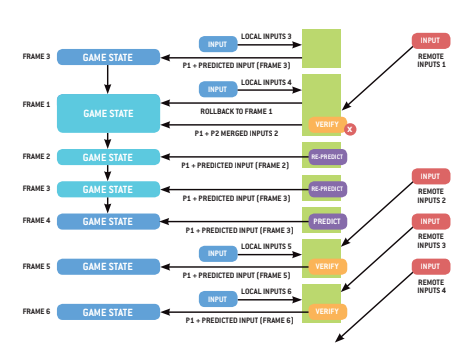
\includegraphics{RollbackNetcodeRepresentation}
\caption{Rollback netcode \cite{GGPODocumentation}}
\label{fig:RollbackNetcodeRepresentation}
\end{figure}
\newpage
\subsection{Difficulties in industry}
In today's fighting game market, many games have rollback \cite{GamesWithRollback}.However there are still notable exceptions such as:
\begin{itemize}
\item Super Smash Bros. Ultimate\cite{SSBU}
\item Granblue Fantasy Versus\cite{GBFV}
\item Under Night In-Birth\cite{UNI}
\item Samurai Shodown\cite{SamSho}
\item Soulcalibur VI\cite{SVI}
\item Dead or Alive 6\cite{DOA6}
\item EA Sports UFC 4\cite{UFC4}
\item Dragon Ball FighterZ\cite{DBFZ}
\end{itemize}

Other fighting games have had difficulty in implementing rollback, such as Street fighter V and Mortal Kombat X.
These difficulties with implementing and developing rollback are the basis of the motivation of this paper.

\subsection{Aim}
To investigate rollback netcode, it's usage in industry and any short comings of existing public rollback netcode infrastructure
\subsection{Objectives}
\begin{itemize}
\item Understand rollback netcode and the effects on the games it's implemented in.
\item Create a visualization for the differences between rollback and delay based netcode.
\item Research the difficulties of implementing rollback in existing games.
\item Explore optimizations for the existing public rollback structure.
\item Investigate further uses of rollback netcode, in the wider video game industry.
\end{itemize}
\newpage
\section{Background}
This section aims to provide information surrounding the different technologies and
concepts which relate to the project objectives. There is a more in depth explaination on the structure of netcode, and some of the common problems it can encounter.

Peer to peer networks over the internet communicate data in packets which can run into the following issues.
\begin{itemize}
\item{Packets take time to reach their destination (Network Latency).}
\item{Packets can get lost on their way (Packet Loss).}
\item{Packets can get there, but have their data corrupted (Corruption).}
\item{Computers can run at different speeds.}
\item{Computers can occasionally get hung up on doing things and skip a frame or two.}
\end{itemize}

\subsection{Delay-based netcode}
\subsubsection{Concept}
Delay based netcode works by keeping both players games in lockstep, meaning that each player's simulation of the game are waits for the input of the remote player, before simulating the frame\cite{DelayBasedNetcode}. This system works well when latency is not a major factor, for example, in a turn based game, where the inputs are spread apart by seconds, a pause of half a second may go unnoticed.
Input latency frames are added to compensate for the Network Latency, and allow the local inputs to be sent before the frame they would be read on as shown in figure \ref{fig:InputLatencyEffect}.

\begin{figure}[h]
\centering
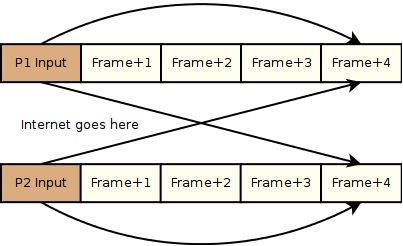
\includegraphics{InputDelay}
\caption{4 Frame Input Delay Example \cite{FightingGameNetworking}}
\label{fig:InputLatencyEffect}
\end{figure}

The Input delay to be used can be calculated as follows:
\[InputLatencyFrames = Ceiling( (RoundTripLatency/2 + Constant) / FrameDuration )\]

Where the constant represents additional frames of delay to compensate for variance in Network Latency.

\subsubsection{Improvements}
However this model does not take into account potential for packet loss/ corrupted packets, which may lead the actual states to progress as shown in figure \ref{fig:PacketLossEffect}

\begin{figure}[h]
\centering
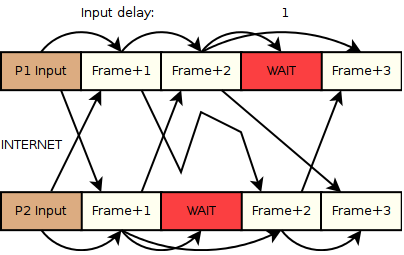
\includegraphics{PacketLossEffect}
\caption{Packet Loss's Affect on Game State progression \cite{FightingGameNetworking}}
\label{fig:PacketLossEffect}
\end{figure}

One unexpected side effect of packet loss with single input packets is knock on delays, where by a delay in one game, makes the frame process later, so the inputs for that frame are postponed, delaying the origins game.

To combat packet loss and data corruption multiple inputs can be sent with one packet, extra frames of input delay can be added, and inputs can be sent multiple times, as shown in \ref{fig:PacketLossSoultions}

\begin{figure}[h]
\centering
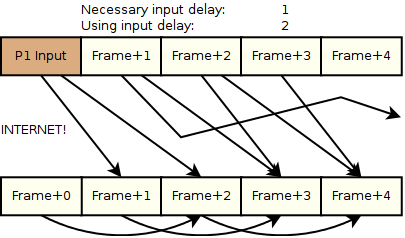
\includegraphics{PacketLossSoultions}
\caption{Potential Solutions to Packet Loss in Delay Based Netcode \cite{FightingGameNetworking}}
\label{fig:PacketLossSoultions}
\end{figure}

Another improvement to made to delay based netcode is to account for Network Latency variance with a dynamic number of delay frames. way to account for Network Latency variance is to have a dynamic number of Delay Frames, varying with average Latency\cite{DelayVsRollback}. This can hide stutters, and remedy degrading network conditions causing consistent pauses. However, consistency for fighting games is the one of the highest determiners on network quality\cite{Core-ARollback}.

\subsubsection{Evaluation}
When there is minimal Network Latency variance, delay based netcode functions similarly to a non networked experience, with increased Input Latency. This is the ideal case for delay based networking. However, when the Network Latency variance is high, the game can freeze at seemingly random moments, removing agency from the player in the middle of a game. This breaks user imersion and significantly decreases the quality of the experience\cite{DelayVsRollback}.

Ultimately Delay based netcode functions as network soultion for high quality connections, but struggles when operating as connection quality degrades. \cite{KIInterview}.
\subsection{Rollback netcode}
Rollback netcode takes the existing framework of delay based netcode and builds on top of it. Instead of waiting for the remote user's input to simulate a frame, the game predicts it.  is These predictive frames By not requiring the input of the remote user to simulate a frame, it can tolerate late and lost packets better than delay based \cite{GGPODocumentation}. When a packet is lost or late, the rollback frames act as a buffer preventing the from game freezing. In theory one could use the rollback buffer to reduce apparent network latency as well. This will be explored later.


max tolerable ping increases
\subsubsection{Difficulties in Implmentation}
- separate gameplay from rendering
- serializable game state
- particle simulation 
- object lifetime 
- sound fx
- animation system
- UI
- desync detection
%\subsubsubsection{One sided Rollback}
%\subsubsubsection{Street Fighter V}
%\subsubsubsection{Mortal Kombat X}
\subsection{Third party Rollback}
- Slippi
- Fightcade

\section{Effects of Rollback on Game Design}
\subsection{8 Frames}
\subsection{Audio Design}
\subsection{Visual Design}


\section{Improvements for Rollback}

I propose a theory for rollback frames 
%rollback = ceiling(sqrt(RTT variance)/frameduration + constant)
%(Only care about upper bound so sd is halved)
%(2 sd's 98.5 could use 3 for 99.95) 
%30(SFV round length) * FPS (60) * 3 (BO3) = number of frames.
%Chance of a 1F stutter = (1-confidance interval)^frames = 


%delay = ceiling ((RTT)/(2*frameDuration) + constant)
for dynamic: dynamically changing rollback = minimal effect, (Problem with maxing rollback?), however try to keep delay static
for static: use upperbound of tolerable network connections (cite Mortal kombat)

\subsection{Prediction Quality}
\subsection{Packet Contents Optimization}
\subsection{Input Locking}

\section{Rollback Visualization tool}
\subsection{Design}

\section{Wider use case of rollback netcode}
Rollback ideas that only apply to fighting games? (Visual teleportation?, Expensive to implement?, ) 
 RTS (Including sports games)

Prediction quality:
- Connection ‘quality’. This doesn’t mean bandwidth, but rather how much a connection’s response time fluctuates. This has improved in modern times, making rollback a much more viable option than it once was.
- The type of game. Because rollback needs you to be able to revert the state of the game in some cases, trying to implement it in a game with hundreds of different units all acting at once is extremely challenging (not to mention very offputting for the player). As a result, it’s more suited to fighting games and other games with fewer player-controlled assets flying around at any given time.

\section{Evaluation}

This section might alternatively be called “Experimental results”.  It describes how you assessed your project and what you found out. Where you give results in tables or graphs, remember to highlight in the text the key points that the data shows and, if possible, try to explain why you got any unexpected results.

\section{Conclusions and further work}

In this section you summarise what you did and discovered and (importantly) what else you would have done (or done differently) if you had the chance. It is a chance to reflect on your success.

\begin{thebibliography}{25}

\bibitem{GGPODocumentation} {\texttt https://drive.google.com/file/d/1nRa3cRBQmKj0-SEyrT\_1VNOkPOJWNhVI/view} or 
{\texttt https://web.archive.org/web/20220101162600/https://drive.google.com/file/d/1nRa3cRBQmKj0-SEyrT\_1VNOkPOJWNhVI/view} 
Tony C., GGPO Game Developer Magazine's article. 2012. (Visited 25/05/2022)

\bibitem{FGCMajors} {\texttt https://liquipedia.net/fighters/Tier\_1\_Tournaments} or 
{\texttt https://web.archive.org/web/20210121113554/https://liquipedia.net/fighters/Tier\_1\_Tournaments} 
Liquidpedia list of major fighting game tournaments. (Visited 25/05/2022)

\bibitem{FirstUSTournament} {\texttt https://www.usgamer.net/articles/the-oral-history-of-evo} or 
{\texttt https://web.archive.org/web/20220321000753/https://www.usgamer.net/articles/the-oral-history-of-evo} 
John L., The Oral History of EVO: The Story of the World's Largest Fighting Game Tournament (Visited 25/05/2022)

\bibitem{FGCAsEsport} {\texttt https://esportsinsider.com/2021/10/can-fighting-games-become-a-mainstream-esport/} or 
{\texttt https://web.archive.org/web/20220516060805/https://esportsinsider.com/2021/10/can-fighting-games-become-a-mainstream-esport/} 
Elizbar R., Can fighting games become a mainstream esport without abandoning grassroots?. (Visited 26/02/2022) 

\bibitem{SmashTournamentsInThePandemic} {\texttt https://www.ssbwiki.com/COVID-19\_pandemic\_and\_its\_impact\_on\_competitive\_Smash} or {\texttt https://web.archive.org/web/20220516020551/https://www.ssbwiki.com/COVID-19\_pandemic\_and\_its\_impact\_on\_competitive\_Smash} List of smash tournaments affected by the pandemic. (Visited 26/02/2022) 

\bibitem{GuiltyGearStriveInThePandemic} {\texttt https://techraptor.net/gaming/opinions/guilty-gear-strive-changed-fighting-games-rollback-netcode} or {\texttt https://web.archive.org/web/20210713144527/https://techraptor.net/gaming/opinions/guilty-gear-strive-changed-fighting-games-rollback-netcode} Davi B. Guilty Gear Strive Might Have Changed Fighting Games Forever. (Visited 26/02/2022)

\bibitem{DelayVsRollback} {\texttt https://arstechnica.com/gaming/2019/10/explaining-how-fighting-games-use-delay-based-and-rollback-netcode/} or {\texttt https://web.archive.org/web/20220425211823/https://arstechnica.com/gaming/2019/10/explaining-how-fighting-games-use-delay-based-and-rollback-netcode/} Ricky P. Explaining how fighting games use delay-based and rollback netcode. (Visted 26/05/2022)

\bibitem{BadNetcode} {\texttt https://www.polygon.com/2020/3/25/21192522/netcode-samurai-showdown-fighting-games-rollback-delay} or {\texttt https://web.archive.org/web/20220401231646/https://www.polygon.com/2020/3/25/21192522/netcode-samurai-showdown-fighting-games-rollback-delay} David C. Bad netcode is killing many of your favorite fighting
games. (Visted 26/05/2022)

\bibitem{RollbackDevelopment} {\texttt https://gamasutra.com/view/news/34050/Interview\_How\_A\_Fighting\_Game\_Fan\_Solved\_Internet\_Latency

\_Issues.php} or {\texttt https://web.archive.org/web/20220325062609/https://gamasutra.com/view/news/34050/Interview\_How\_A\_Fighting\_Game\_Fan\_Solved\_Internet\_Latency\_Issues.php} Kyle O. Interview: How A Fighting Game Fan Solved Internet Latency Issues. (Visted 26/05/2022)

\bibitem{FightingGameDefine} {\texttt https://archive.org/details/nextgen-issue-015/page/n33/mode/2up} "The Next Generation 1996 Lexicon A to Z: Fighting Game". (Visited 26/05/2022)

\bibitem{DelayBasedNetcode} {\texttt https://www.gamasutra.com/view/feature/3094/1500\_archers\_on\_a\_288\_network\_.php} or {https://web.archive.org/web/20220506231117/https://www.gamasutra.com/view/feature/3094/1500\_archers\_on\_a\_288\_network\_.php} Mark T. 1500 Archers on a 28.8: Network Programming in Age of Empires and Beyond. (Visted 26/05/2022)

\bibitem{FightingGameNetworking} {\texttt https://web.archive.org/web/20210228051849/https://mauve.mizuumi.net/2012/07/05/understanding-fighting-game-networking.html} Mauve M. Understanding Fighting Game Networking. (Visted 26/05/2022)

\bibitem{GamesWithRollback} {\texttt https://attackofthefanboy.com/guides/rollback-netcode-games-list/} or {\texttt https://web.archive.org/web/20211122034207/https://attackofthefanboy.com/guides/rollback-netcode-games-list/} Andron S. Rollback Netcode Games List (March 2022). (Visted 26/05/2022)

\bibitem{SSBU} {\texttt https://en.wikipedia.org/wiki/Super\_Smash\_Bros.\_Ultimate} or {\texttt https://web.archive.org/web/20220519200835/https://en.wikipedia.org/wiki/Super\_Smash\_Bros.\_Ultimate} Super Smash Bros. Ultimate. (Visited 26/05/2022)

\bibitem{GBFV} {\texttt https://en.wikipedia.org/wiki/Granblue\_Fantasy\_Versus} or {\texttt https://web.archive.org/web/20220512125807/https://en.wikipedia.org/wiki/Granblue\_Fantasy\_Versus} Grandblue Fantasy Versus (Visited 26/05/2022)

\bibitem{UNI} {\texttt https://en.wikipedia.org/wiki/Under\_Night\_In-Birth} or {\texttt https://web.archive.org/web/20220516020108/https://en.wikipedia.org/wiki/Under\_Night\_In-Birth} Under Night In-birth (Visited 26/05/2022)

\bibitem{SamSho} {\texttt https://en.wikipedia.org/wiki/Samurai\_Shodown\_(2019\_video\_game)} or {\texttt https://web.archive.org/web/20220504020927/https://en.wikipedia.org/wiki/Samurai\_Shodown\_(2019\_video\_game)} Samurai Shodown (Visited 26/05/2022)

\bibitem{SVI} {\texttt https://en.wikipedia.org/wiki/Soulcalibur\_VI} or {\texttt https://web.archive.org/web/20220421074040/https://en.wikipedia.org/wiki/Soulcalibur\_VI} Soulcalibur VI (Visited 26/05/2022)

\bibitem{DOA6} {\texttt https://en.wikipedia.org/wiki/Dead\_or\_Alive\_6} or {\texttt https://web.archive.org/web/20220130144906/https://en.wikipedia.org/wiki/Dead\_or\_Alive\_6} Dead or Alive 6 (Visited 26/05/2022)

\bibitem{UFC4} {\texttt https://en.wikipedia.org/wiki/EA\_Sports\_UFC\_4} or {\texttt https://web.archive.org/web/20211019192531/https://en.wikipedia.org/wiki/EA\_Sports\_UFC\_4} EA Sports UFC 4 (Visited 26/05/2022)

\bibitem{DBFZ} {\texttt https://en.wikipedia.org/wiki/Dragon\_Ball\_FighterZ} or {\texttt https://web.archive.org/web/20220424200258/https://en.wikipedia.org/wiki/Dragon\_Ball\_FighterZ} Dragon Ball FighterZ (Visited 26/05/2022)

\bibitem{Core-ARollback} {\texttt https://www.youtube.com/watch?v=0NLe4IpdS1w} or {\texttt https://web.archive.org/web/20220529231214/https://www.youtube.com/watch?v=0NLe4IpdS1w} Core A Gaming. Analysis: Why Rollback Netcode Is Better. (Visted 31/05/2022)

\bibitem{KIInterview} {\texttt https://www.youtube.com/watch?v=1RI5scXYhK0} or {\texttt https://web.archive.org/web/20220330062542/https://www.youtube.com/watch?v=1RI5scXYhK0} Hold Back To Block. Talking Netcode With Adam "Keits" Heart (Visited 31/05/2022)

\bibitem{InputLatencyDatabase} {\texttt https://displaylag.com/video-game-input-lag-database/} or {\texttt https://web.archive.org/web/20220519183335/https://displaylag.com/video-game-input-lag-database/} Display Lag. Video Game Input Lag Database. (Visted 02/06/2022)

\end{thebibliography}
\end{document}
